\section{Exploring the Design Space of Text Input in VR}

\subsection{Challenges of Text Entry in Virtual Reality}

An average person can type between 38 to 40 words per minute, thanks to the dexterity of our fingers, the haptic feedback from the physical keyboards, and visual feedback on the display.    In the context of virtual reality, it is often not an option to use a physical keyboard.  We are usually not sitting down and it is hard to switch between the VR controllers and a physical keyboard, further complicated by the fact that we cannot see the keyboard in VR. It is desirable to be able to type with existing VR input devices, so we don’t have to remove the head gear to type. 

\subsubsection{Latency in Visual Feedback}
Typing is complex interaction that requires a high-bandwidth feedback loop~\cite{McGill:2015:DRO:2702123.2702382}.
Latency is a barrier in achieving a seamless interaction between the real and virtual~\cite{leedesigning}.

In virtual reality, latency is the time between movement of the user's head and the updated image being displayed on the screen.  
This includes time includes the times for fusion, image transmission,
rendering, sensor response and display response.
This is commonly referred to as the \textit{motion-to-photon} latency.

To achieve a genuine sense of presence~\cite{schuemie2001research} in virtual reality, the total \textit{motion-to-photon} latency must be less than 20 milliseconds~\cite{jerald2009relating,jerald2010scene,bailey2004latency} for head movement.
Some existing systems have a latency as high as 80 milliseconds ~\cite{lincoln2016motion,dallaire2016animated}.

Touch-based interactions need even tighter tolerances on latency compared to head movement described above.
Research on touchscreens finds that for a user to perceive display elements as naturally being affected by touch, there is a perceptual floor between 2  and 11 milliseconds below which users do not notice lag~\cite{Jota:2013:FFE:2470654.2481317,Ng:2012:DLD:2380116.2380174}.
Further, it is found that latencies down to 2.38 milliseconds are required to alleviate user perception when dragging~\cite{Jota:2013:FFE:2470654.2481317,Ng:2012:DLD:2380116.2380174}.

\subsubsection{Proprioception}
The most prominent problem for a traditional keyboard in a virtual environment setting is that the user cannot see the actual keyboard that he or she is using or his own finger.
Manipulation in virtual reality is difficult because users must do without the haptic contact with keyboard buttons they rely on in the real world to orient themselves.

\subsubsection{Muscle Fatigue and Dexterity}

Haptic feedback and physical constraints in real world input devices help to define interactions. 
Fine-grained control is difficult in virtual reality and restricts users to the coarse manipulation of virtual objects.
Input devices that excluded the use of the fingers are slower~\cite{Zhai:1996:IMG:238386.238534}.  
Midair interactions are prone to fatigue and lead to a feeling
of heaviness in the upper limbs~\cite{Hincapie-Ramos:2014:CEM:2556288.2557130}, commonly known as the \textit{gorilla arm effect}.

\subsection{Initial Experimentation}

Our exploration of VR input methods started by building a few prototypes and asking 3-5 users to type a few sentences with the prototyping.  
The users was given little to no instruction about how the input device worked.
The goals of this process was to explore the performance potential of each input device and to investigate if users could understand the visual interface.
We record how long the input took, their understanding of the input device, and their other feedback.

\subsection{Design \#1 - Gaze Input}
Most VR apps today use gazing as an input method.  A virtual keyboard is presented in VR, and users type a letter by gazing at the desired key and tapping on the gear or controller.  Not only did the users find the process slow, but it also causes nausea as they tap the head gear. 
The user can type about 10 words per second. [CHECK]  

\subsection{Design \#2 - Drumming}
Google models typing as drumming.  Users use the VR controllers as drumsticks; typing a character means hitting the right drum among the set of 26 drums laid out like a keyboard. Users found that it was fun initially, but soon discovered that it is very hard to hit the right key.   The user can type about 10 words per second. [CHECK!!!]
It is also easy to get tired. 
Both Designs \#1 and \#2 support the use of fingers touching a physical device in text entry. 

\subsection{Design \#3 - External Camera}

We next explore the use of a virtual keyboard on a touchpad, the input method used on mobile phones today.  To address the problem that we cannot see our fingers in virtual reality, we experimented with mixed reality (augmented plus virtual) with a camera.  Our prototype points the front facing camera on the head mounted display points at the mobile keyboard, and streams the view of our fingers and the keyboard into the virtual environment. 

The goal of this prototype is to investigate how latency and presence, particular of the fingers, affect performance.  We found that the latency is an inhibitor to fast input.  Our fingers are so fast that we can only see where our fingers were.  What we see is constantly wrong and just makes it even harder to type.  This prototype demonstrates how challenging the visual latency is for typing. 

\subsection{Design \#4 - 26-key Tap}
\vspace*{.1cm}
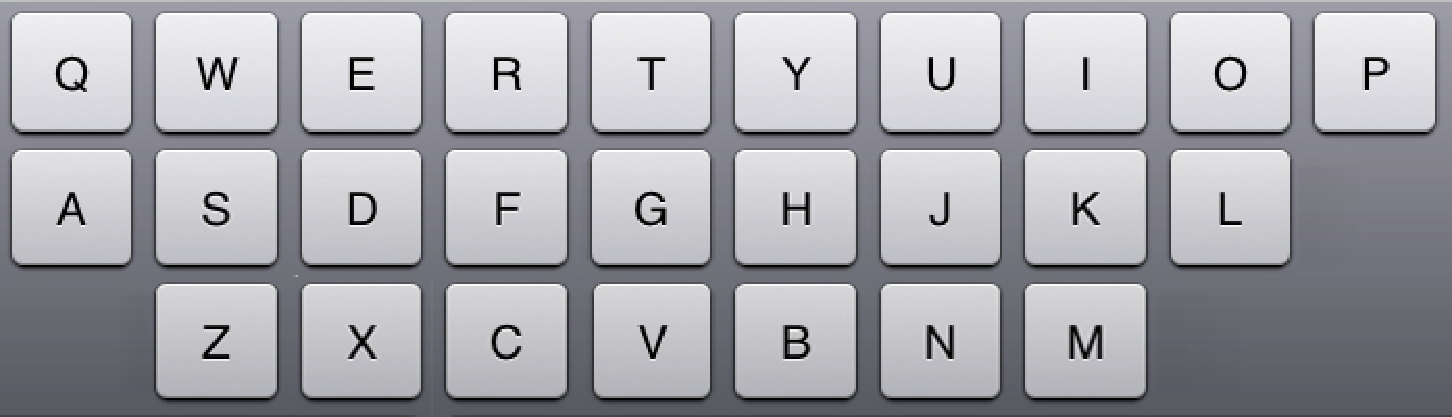
\includegraphics[width=.9\columnwidth]{figures/26Tap}

In this experiment, we explore the use of a regular mobile keyboard.  The prototype projects the keyboard and the keys touched onto the virtual environment, and also shows the letters typed in a textbox.  The keys are laid out exactly as a regular mobile keyboard. 
Aggressive autocorrect algorithm adjusted for typos and phonetic misspelling are applied.
The advantage of such keyboard is that users do not need to change their interaction with a keyboard at all.  Users are familiar with typing on the mobile device; some even can type with both thumbs.  

We noticed an unexpected phenomenon using this prototype.  Even hitting the same key twice is difficult.  Every time a user lifts a finger and lowers the finger, there is a nontrivial chance that the finger has drifted to another key.  Even though the keyboard layout is familiar, and even if error correction has been successful in speeding up text entry on mobile devices, it is hard to enter a sentence correctly.   

\subsection{Design \#5 - 26-key Swipe}
\vspace*{.1cm}
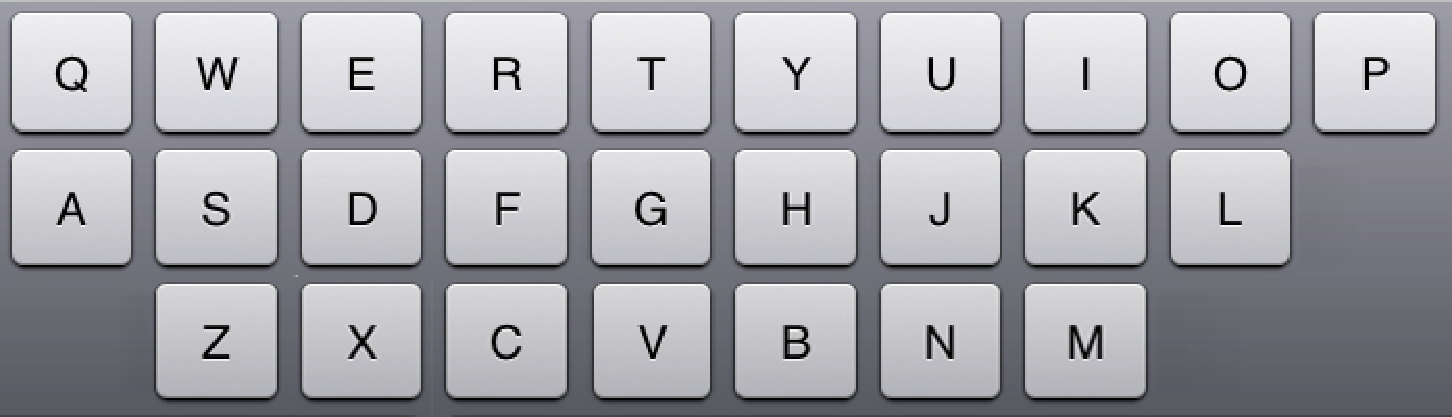
\includegraphics[width=.9\columnwidth]{figures/26Tap}

Swiping has been shown to be effective in speeding up typing on mobile devices.  Since it does not involve lifting the finger, we postulated that it may also be appropriate for VR.  
Similar to the 26-key tap, the layout of the mobile QWERTY keyboard is preserved, except tapping is replaced by dragging to specific keys.  We show on the virtual keyboard a trail to indicate where the finger was.  Same autocorrect algorithm is applied.   Swiping works much better than tapping.  However, there are two main problems: 
\begin{enumerate}
\item
Users cannot get the first letter right. 
\item
The speed with which the user seeks the appropriate key is much slower than on the soft keyboard on the mobile device because of the lag in visual feedback. 
HOW FAST? 
\end{enumerate}

In summary, the use of swipe over a conventional keyboard is the best among the choices we explored in the initial phase.  Nonetheless, the speed of XYZ-CHECK is still much lower than desired. 


\begin{comment}
>
\subsection{Design \#4 - 8-key Drag}
\vspace*{.1cm}
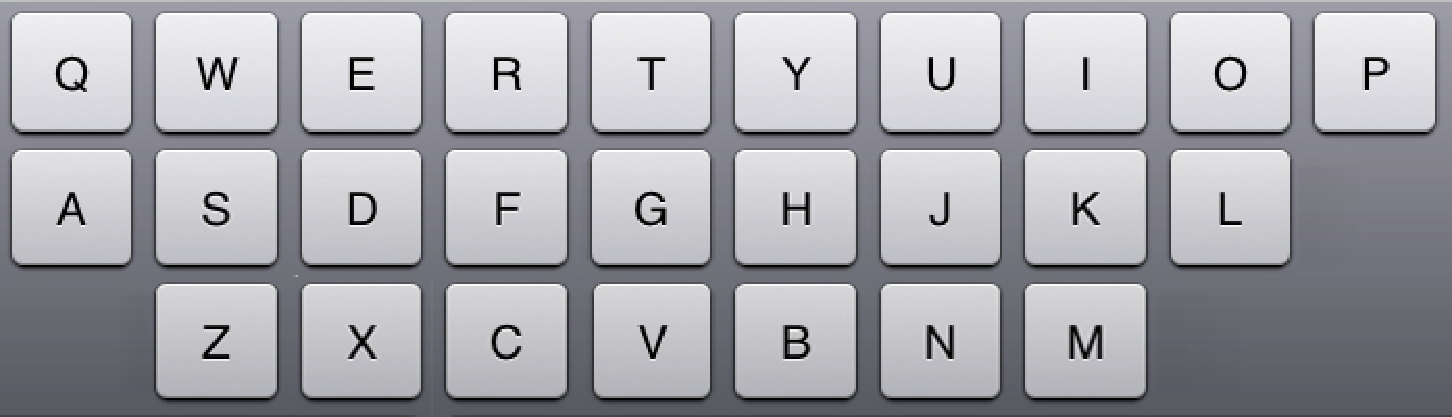
\includegraphics[width=.9\columnwidth]{figures/26Tap}

QWERTY keyboard is broken into 8 regions instead of 6.
User interact with this keyboard through dragging.
Both hands are required, with each hand dragging four directions (left, up, right, down) to input the 8 regions.

\subsection{Design \#5 - 6-key Tap}
\vspace*{.1cm}
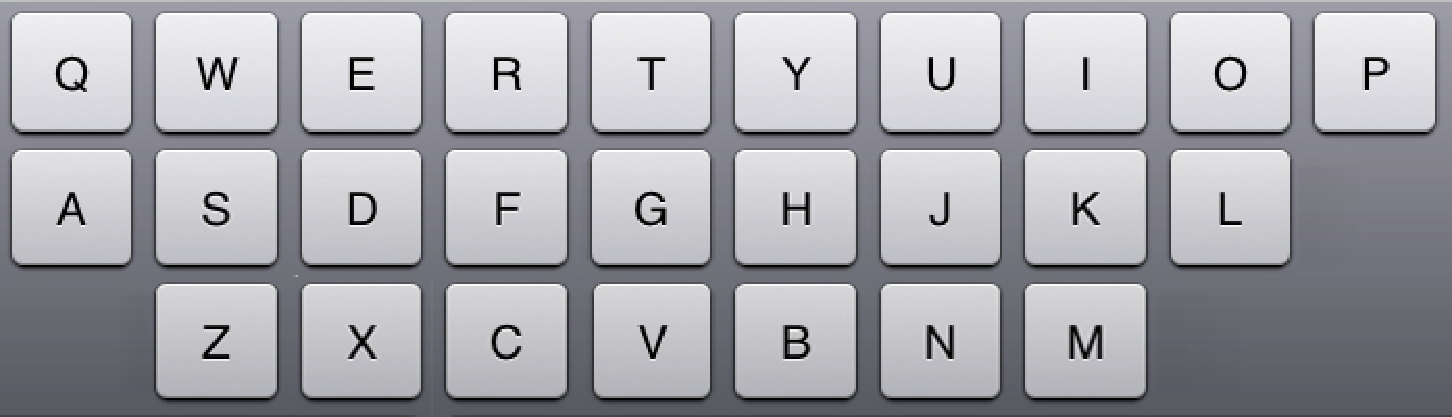
\includegraphics[width=.9\columnwidth]{figures/26Tap}

This is our first design utilizing batched keys. QWERTY keyboard is divided into 6 sections. Tapping corresponding regions triggers input for a whole section.
A word recommender algorithm in back end is required.


\subsection{Design \#6 - 6-key Drag}
\vspace*{.1cm}
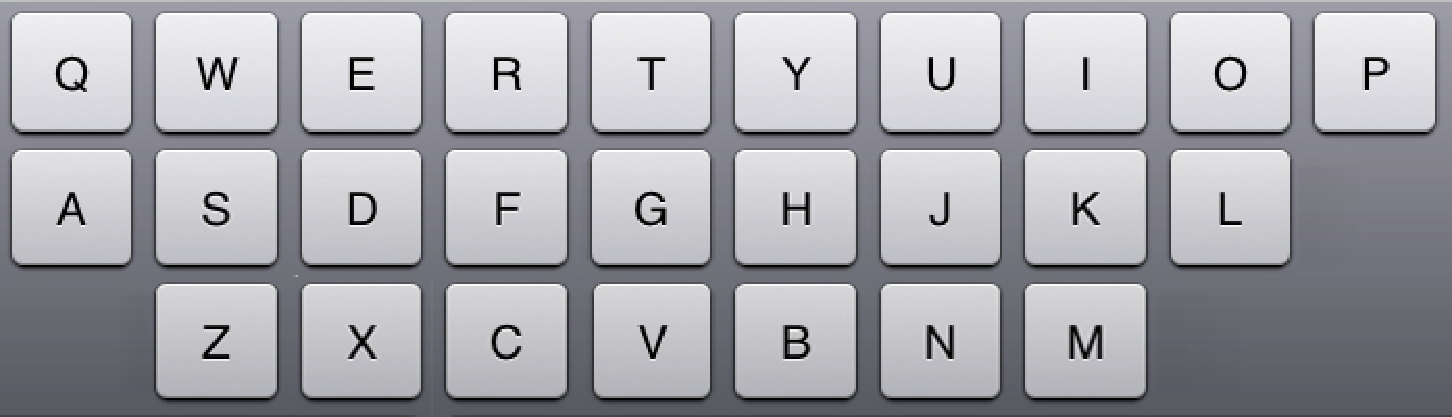
\includegraphics[width=.9\columnwidth]{figures/26Tap}

Similar to 6 keys tap, the method of interaction is changed to drag instead of tap.
A word recommender algorithm in back end is required.

Even though there can be realistic representation of the keyboard and his fingers in VR, users still suffer from not being able to see some part of his own body.
The solution to such visual segmentation is not apparent, for whole body tracking in VR is not yet available.

Studies show that users possesses approximate knowledge of where their fingers are on screen thanks to proprioception \cite{boff1986handbook}.

\section{Design Goals}
Before describing the prototypes and lessons learned, we present five high-level design goals that focus on input metrics, user experience, and adaptability.
These goals are informed by related work and our experience building other systems.

\subsection{Efficient}
How closely does the new device approach exceed the speed of the best devices for text input in virtual reality?

\subsection{Learnable}
How long does the device take to learn?
Does it rely on existing skills?
Is there ways for the user to transition from being a novice to an expert?

\subsection{Practical}
Is the input method usable today?
Moreover, will it be usable in the future given the where we think virtual reality controller are heading?

\subsection{General}
Is the text input method useful across multiple types of applications?
Can the user type their username, password, and a message to a friend?

\subsection{Usable}
Desktop user sessions are longer than mobile~\cite{Kamvar:2009:CIM:1526709.1526817}.
We hypothesize that virtual reality will have a user session time closer to that of a desktop computer than a mobile phone.
Once a user has take the time to wear the head mounted display and controller, the session will
Will the user be able to use the text input method comfortably?
Can they use it for as long as they use as they their computer at night?


\end{comment}

